%
% Refrence http://en.wikibooks.org/wiki/LaTeX
%

\documentclass[10pt]{article}

% ======
% Header
% ======

% use droid sans
\usepackage{droidsans}    
\renewcommand\familydefault{\sfdefault}   % set default font to sans-serif


% enable \href
\usepackage[colorlinks=true,
            linkcolor=blue,
            urlcolor=blue,
            allbordercolors={0 0 0},
            pdfborderstyle={/S/U/W 1}]{hyperref}

% enable \includegraphics for embedding jpgs
\usepackage{graphicx}  

% ==================
% Document Meta Data
% ==================

\title{Webtech Report}
\author{Imna Malik n James Sewart}
\date{29-5-16}

% ====
% Body
% ====

\begin{document}

    \maketitle

    \tableofcontents


    \begin{abstract}
        visual music discovery service using data crawled from various apis and combined
    \end{abstract}

    \section{Client}
        \subsection{Style}
            \subsubsection{General Layout}
                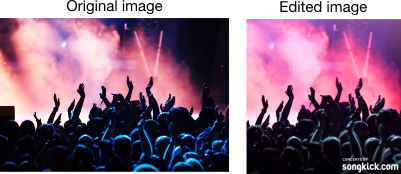
\includegraphics[height=60mm]{example2.png}

                The web app consists of a single page which is filled with a map using the google maps api. There are two panels: the search on the left, and the info panel on the right. 

                The search panel consists of an input to type a query and two date pickers to choose the date range for events to be displayed. When a search query is made, results are shown underneath with the date of the event, the band names that matched, and the time to walk their if available.

                The info panel slides in from the right when selecting an event, either through a map marker or a search item. It includes one or more artist thumbnails at the top depending on how many artists are playing that event. Underneath is the artist name, image, and biography for the currently selected artist. Next is an embedded Spotify player for that artist that is revealed by pressing the play button. Further is information about the events venue and link to the ticket purchasing page.

                The pink markers on the map represent events and the purple marker is the users current location determined by the browser.

                The info panel will slide away when the map is moved or zooms. When the info panels content overflows the bottom of the page it will be scrollable independent of the whole page.


            \subsubsection{Base Classes}
                The design of our layout is inspired by Material Design, using card style boxes. Each panel is given a shadowbox class which gives the element a border radius, shadow, slight transparency, and a dark background colour. The search panel and all panels in the info bar are given this class.

            \subsubsection{Resizing}
                We use CSS media queries to resize the info panel stuff like the and basically and the seearch panel thats everything. The font resize thingy we use percentages and ems we basically use the media query thing we change the font size and have everything inside percentages so everythings dynamic

                We use CSS media queries to change large scale layouts based on the screen size. There are three of these: mobile-sized, large, and extra large. These changes involve setting the widths of the main panels such that they look good on the screen size. For the mobile screen this means the panels are full width and stack on top of each other. For the large size the info bar takes up a third of the screen, and the search 40\% of the screen.

                For a more dynamic resize control we subscribe to the onresize event of the window and scale the whole documents font size based on the screen width. Most elements are defined using ems and so they all scale accordingly.

            \subsubsection{Info Panel}
                The info panel involves many different styling and scripting elements. The panel is animated in using the css transition property and setting the margin-right to 0 from -33\%. By default moving this panel to the right would bring up a scrolling bar however this is disallowed by setting overflow to hidden for the body.

                In order to get the desired scrolling effect we set the overflow-y to scroll which allows the contents to scroll within this div. The height is set to 100\% of the screen height so the content will never increase the full page size.

                The artist thumbnails are contained within an element with text-align set to centre. Each image is an inline-block which means they overflow and stay centred no matter how many artists are inserted. As the images they contain could be of any aspect ratio and we want the thumbnail to be square, we use the object-fit css property to keep the container box filled with the image inside. The containing box is given a border radius of 50\% to make it circular, and the overflow is set to hidden to crop the image inside. The thumbnail is animated to zoom on hover using a css selector that transforms the scale of the container.

                The missing artist picture was created by importing an image found online into inkscape with the image rendering mode set to smooth. Then an avatar silhouette was overlayed on top of it.

                The second box down includes an element for the artist title, along with a paragraph tag for the biography. The title is overlayed onto the the artist image and has a gradient behind in order to make sure the text is visible. The title is pinned to the bottom of the image. The image width is set to the parents width so that only the height changes depending on the aspect ratio of the image. this height will push down the biography. Padding is set on the biography for visual aesthetic.

                The next box contains a self made svg that when clicked, triggers a set of animations. The two triangles will turn 120 degrees with slightly different durations using SMIL animations, the background colour of the box fades from purple to grey, and the size of the box increases to reveal an iframe with a spotify player inside. These animations are reversed on second click to hide the player. when updating the info panel, the url for the iframe is updated with the current artists uri, this triggers that url to be loaded inside, causing the correct player to be displayed.

                This svg was created using the inkscape polygon tool to make a filled triangle. Then by duplicating the triangle and enlarging it then excluding we get a stencil triangle. Then simply by making a same sized triangle and offsetting its psition we get the desired effect.

                The final two boxes display information about the venue. The first displays the venue title and its address. Clicking this will open a new tab with the songkick venue page. The second box holds another self made svg of tickets. Clicking this will take you to the songkick ticket purchasing site.

                Starting with a rectangle we rounded the corners. Making two squares for each end with rounded corners, we used the difference tool to cut out a semi-circle. By duplicating a rectangle with rounded corners 5 times and combining them using the combine tool for simplicity. Using this combined object we exclude the shape from the ticket. Then we tried duplicating the svg and using the outset tool to make one bigger, then aligning the two and using the exclusion tool we get the stencil ticket. This didn't quite have the desired shape so instead we scaled the second ticket and extruded these two. This gives near uniform line thickness. Then by placing the stencil over a copy of the original and using the difference tool we cut a shadow. Now by simply placing the stencil in the gap we produced the desired svg. 

                The background image for the ticket button was taken online and edited using gimp. First the image was cropped to be square. Using the colour balance tool we adjusted the shadows, midtones, and highlight to make the pink and blue stand out. Next using the hue tool we modify the pink to match the websites colour scheme. Other colours were reduced using this tool. Next using the curve tool we adjust the rgb channels so that the image is more aesthetically pleasing. Next we created a new pink layer and layer mask for that layer. Using the gradient tool set to black to white we add a gradient to the mask which adds a pink gradient to the image. This is done twice, once to add a pink gradient that is prominent at the top, and one with a black gradient that is prominent at the bottom to produce a vignette effect. Next using the fuzzy tool with feathered edges to select the people in the image and using the hue/saturation tool, the blues were adjusted to be more grey using the overlap setting to consider overlapping hue values. Next we added the songkick watermark as an overlapping layer, positioning it in the bottom right layer and resizing as desired.

                When a user hovers their mouse over the lower two boxes, an animation is triggered to dim the image. This is achieved using an anchor html tag that is given the class boxClickUrl that expands the anchor to cover the entire parent. The dim effect is achieved by setting the opacity of the image to a smaller value, revealing the black shadowbox behind.

            \subsubsection{Search Panel}

                \begin{itemize}
                    \item persistent search box with icon from a custom font
                    \item the google maps distance matrix api is used on the client side to determine how far away events are from the users current location, this is displayed with the search
                    \item a custom date icon was created using html and adds a nice visual to when event takes place, this is generated by javascript with the date and month injected in to be added to each search result
                    \item clicking on a search result repositions the map to see where it is and opens the relevant info panel
                \end{itemize}

            \subsubsection{Date Filter}
                \begin{itemize}
                    \item fixed up real nice calendar lib and made pull request n all \textless3
                    \item looks super dank in the search panel iluvit
                \end{itemize}

            \subsubsection{Map}
                \begin{itemize}
                    \item using the google maps api with a custom theme
                    \item adding markers for each event in our data structure
                    \item marker onclick opens the info bar for the desired event and centers the event, also animated the marker icon using googles animations
                    \item the marker icons are a custom svg designed by imna herself
                \end{itemize}


        \subsection{Logic}
            There exists one script for all the logic of the webapp. We subscribe to the window onload event as well as the google map callback. In the window load event we setup a few things, including setting up the callbacks for the svg button, initialising the websocket to the server, and initialising the date filter boxes.

            When the map has loaded, we request the browsers location via the google maps api and setup the markers on the map. After both the map has loaded and the websocket has loaded we send the user location to the server via the websocket. This triggers the server to find nearby events to be send back to the client.

            When an array of events arrive we populate our internal events array and initialise the marker for each event. A query is made to find the walking time to each of the events as well. Once this has happened the user can click on the markers to open up the information for the event, as well as being able to search for events using the search bar.
            \begin{itemize}
                \item the main script initiates a websocket connection with the server, and once both the map and the websocket connection is made, the client sends its current map position to the server.
                \item This triggers the server to send nearby events, which once received are visualised on the map as our custom markers.
                \item a user can then click a marker which triggers the sidepanel to be animated in and its content updated to match the information in the data structure for that event
                \begin{itemize}
                    \item this involved creating a dynamic number of band thumbnails and inserting it into the correct position
                    \item updating the band info box to the first band name and description, as well as updating the spotify player with the bands spotify link
                \end{itemize}
                \item the event name and location is updated as well as the links to the event page and the ticket buying page

                \item keyup in the search bar triggers search algorithm on nearby events which generates the results html
                \item results html is inserted inside a container div that is already there
                \item the search algorithm performs a sublime like fuzzy search by not matching sequential matches but each character can match any length into the text
                \item each matched character is given the bold html tag to signify that is the character that matched
            \end{itemize}

    \section{Server}
        The server uses the provided script with modifications. The index is served as a static file and dynamic content is achieved using Websocket connections between the client and server. This design choice simplifies the file resource serving logic, reducing the dynamic parts to message passing.

        Once the client has initialised the webpage, it sets up a secure Websocket connection to the server. A secure socket is preferred as non secure sockets are disallowed when viewing the page over https. The connection is abstracted into websocket.js such that server.js can simply pass a callback that is called when a new client query is made, with a parameter that can be called with the result to send back. server.js doesnt need to worry about managing connections.

        The client will query the browser for its current geographical location and when given, will send this to the server along with a desired date range. The server will reply at some point in the future with an array of events.

        The server will receive this data and use it to query the database using a geoNear query on a \href{https://docs.mongodb.com/manual/core/2dsphere/}{2dsphere} index, and a date range query on the event date. The results are sent to the client.

        Websockets provide a stream of messages, where a message is either some binary data or a string. We serialize JSON for sending data between the client and server. When the client sends its position and desired date range we serialize a data structure that looks like the following.

        \begin{verbatim}
        {
            pos: {
                lat: Number,
                lng: Number
            },
            dateRange: {
                from: Date,
                to: Date
            }
        }
        \end{verbatim}

        Dates aren't parsed into JavaScript date objects when using a JSON.parse so these are handled manually for the database queries.

        As well as giving the client the desired data we have, we also check whether the database needs updating. The data is collected using a variety of APIs. First we ask songkick for the area that the user is in, this allows us to check the database to see if we have checked this area at all/recently. If we haven't got an up to date set of events for this area, we start downloading the events for the area as well as querying last.fm for the artists biography and picture, spotify for a reference to their spotify page, and googles reverse geocode api to get the full address of the venue.

        For each area we limit the speed of requests in order to avoid rate limiting. Any returned errors by the APIs are handled graciously. Once complete data about an event is retrieved, it is stored in the database using an \href{https://docs.mongodb.com/manual/reference/method/db.collection.update/#upsert-option}{upsert} on the event title, to either update an already queried event, or insert as a new event.

        A possible optimization of the client-server interaction process would be to determine what events have already been sent to the client in order to avoid sending them again if they only scroll the map slightly. This would allow for significantly less data to be transferred between the two and would avoid reprocessing every event on the client side on every query change.


    \section{Deployment}
        \begin{itemize}
            \item by default server connects to a local mongodb instance and runs on the latest nodejs.
            \item This favours a vps installations on services like digitalocean or aws by simply cloning the git repo, performing an npm install and running both mongodb and the server script.
            \item the site is live at https://smple.uk
            \item git
        \end{itemize}

    \section{API}
        \begin{itemize}
            \item We made efforts to abide by the api tos by rate limiting and providing * where requested
            \item songkick-spotify-google-last.fm
            \item last.fm requires a link to their site when using their data, biographies always include  a link to last.fm
            \item songkick requires attribution which was intergrated into the ticket logo
        \end{itemize}


    % \begin{verbatim}
    %     j = []
    %     for i in range(10):
    %       j.append(i)
    %       j.append(i+1)
    %       j.append(i+2)
    %     sum(j)
    % \end{verbatim}


    % \subsection{Raw pictures}
    % \includegraphics[height=60mm]{moon.jpg}

    % \subsection{Figures}
    % \begin{figure}[!ht]
    %   \centering
    %     \reflectbox{%
    %       \includegraphics[width=0.5\textwidth]{moon.jpg}}
    %   \caption{A picture of the same gull
    %            looking the other way!}
    % \end{figure}

    % \section{Hyperlinks}
    % \href{http://www.google.com}{Ut enim}

    % \section{Tables}

    % \begin{tabular}{ l | c | r }
    %   \hline
    %   1 & 2 & 3 \\ \hline
    %   4 & 5 & 6 \\ \hline
    %   7 & 8 & 9 \\ \hline
    % \end{tabular}


    %
    % Footnotes
    % 
    % \section{Footnotes}
    % This is an example footnote\footnote{An example footnote.}
    % \footnotetext[17]{This is my footnote!}

    % \footnotemark[17]




\end{document}


